%------------------------------------------------------------------------------
%  DOCUMENT CONFIGURATION
%------------------------------------------------------------------------------

\documentclass[twoside, a4paper, titlepage]{article}
\usepackage[landscape]{geometry}

%------------------------------------------------------------------------------
%  PACKAGES
%------------------------------------------------------------------------------

\usepackage{graphicx} % Required to insert images
\usepackage{rotating} % Required for sideways figure
\usepackage{parskip} % Required for paragraph styling
\usepackage{float} % For having figures inline
\usepackage{amsmath}
\usepackage{amssymb}
\usepackage{hyperref} % For links
\usepackage{blindtext}
\usepackage{outlines}
\usepackage{tabularx}

\usepackage{tikz}
\restylefloat{figure}

\begin{document}

% Definition of blocks:
\tikzset{%
  block/.style    = {draw, thick, rectangle, minimum height = 3em,
    minimum width = 3em},
  sum/.style      = {draw, circle, node distance = 2cm}, % Adder
  input/.style    = {coordinate}, % Input
  output/.style   = {coordinate} % Output
}

\pagestyle{empty}

%------------------------------------------------------------------------------

\begin{figure}[H]
  \centering
  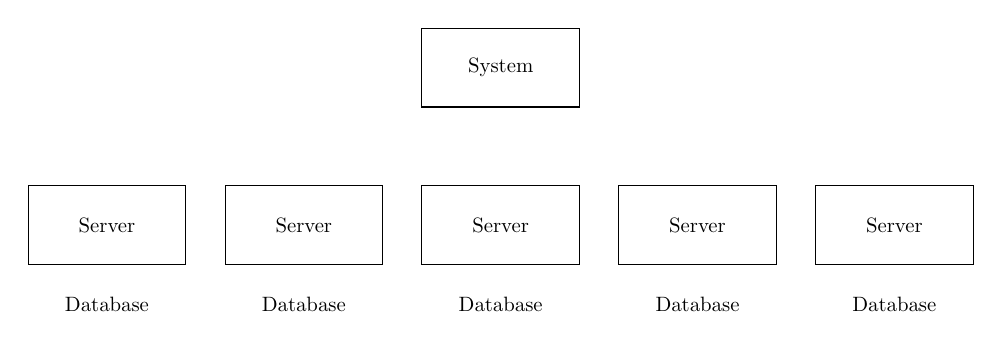
\begin{tikzpicture}[scale = 0.5, every node/.style={scale = 0.75}]

  \node[align=center] at (0, 0) {System};
  \draw (-2, 1) rectangle (2, -1);

  \node[align=center] at (-10, -4) {Server};
  \draw (-12, -3) rectangle ( -8, -5);

  \node[align=center] at (-10, -6) {Database};

  \node[align=center] at ( -5, -4) {Server};
  \draw ( -7, -3) rectangle ( -3, -5);

  \node[align=center] at ( -5, -6) {Database};

  \node[align=center] at (  0, -4) {Server};
  \draw ( -2, -3) rectangle (  2, -5);

  \node[align=center] at (  0, -6) {Database};

  \node[align=center] at (  5, -4) {Server};
  \draw (  3, -3) rectangle (  7, -5);

  \node[align=center] at (  5, -6) {Database};

  \node[align=center] at ( 10, -4) {Server};
  \draw (  8, -3) rectangle ( 12, -5);

  \node[align=center] at ( 10, -6) {Database};


  % % AWS Architecture
  % \draw (-1, -1) rectangle (11, 11);
  % \draw (0, 0) rectangle (4, 4);
  % \draw (6, 0) rectangle (10, 4);
  % \draw (3, 6) rectangle (7, 10);
  % \draw[dashed, very thick, green] (4.75, 10.5) -- (8.75, 14);
  % \draw[dashed, very thick, green] (5.25, 10.5) -- (9.25, 14);
  % \draw[dashed, very thick, green] (7.5, 8.25) -- (13, 5.25);
  % \draw[dashed, very thick, green] (7.5, 7.75) -- (13, 4.75);
  %
  % % Ethereum
  % \draw (12, -1) rectangle (18, 11);
  % \draw (13.5,  3.5) rectangle (16.5, 6.5);
  %
  % % Front-end services
  % \draw (7, 13) rectangle (11, 17);
  % \draw[dashed, very thick, green] (8.75, 14) -- (14.75, 7);
  % \draw[dashed, very thick, green] (9.25, 14) -- (15.25, 7);
  %
  % \node[align=center] at (2, 2) { RDS\\SQL-based DB };
  % \node[align=center] at (8, 2) { S3\\Distributed File\\System };
  % \node[align=center] at (5, 8) { EB\\Scalable API };
  %
  % \node[align=center] at (9, 15) { Multiple\\front-end clients };
  %
  % \node[align=center] at (15, 5) { Public\\Ethereum\\Cluster };

  \end{tikzpicture}
  \caption{
    System structure representation using client, database, replica, server, and system modules.
  }
\end{figure}

%------------------------------------------------------------------------------

\end{document}
